\documentclass{article}

\usepackage[english]{babel}     
\usepackage[utf8]{inputenc}     % accent symbols
\usepackage[T1]{fontenc}
\usepackage{lmodern}
\usepackage{microtype}
\usepackage{natbib}
\usepackage{tocbibind}          
\usepackage{amsmath}            % math symbols
\usepackage{amsthm}             % math symbols
\usepackage[colorlinks=true,linkcolor=red]{hyperref} % hyper link

% for code
\usepackage{listings}
\usepackage{color,xcolor}
\definecolor{mygreen}{rgb}{0,0.6,0}
\definecolor{mygray}{rgb}{0.9,0.9,0.9}
\definecolor{mymauve}{rgb}{0.58,0,0.82}
\lstset{
backgroundcolor=\color{mygray},
numbers=left,                    
columns=fullflexible,
breaklines=true,      
captionpos=b,         
tabsize=4,            
commentstyle=\color{mygreen}, 
escapeinside={\%*}{*)},       
keywordstyle=\color{blue},    
% stringstyle=\color{mymauve}\monaco,
frame=single,                        
rulesepcolor=\color{red!20!green!20!blue!20},
% identifierstyle=\color{red},
%% language=c++,
basicstyle=\tiny
}

\usepackage{indentfirst}
\setlength{\parindent}{2em}
\usepackage[onehalfspacing]{setspace}
% graph
\usepackage{pdfpages}
\usepackage{graphicx}
% box
\usepackage{booktabs}
\usepackage{tcolorbox}

%% user defined command
\newcommand{\keyword}[1]{\textbf{#1}}
\newcommand{\keywords}[1]{\textbf{#1}}
\newcommand{\lcmd}[1]{\texttt{#1}}
\newcommand{\head}[1]{\textnormal{\textbf{#1}}}
\newcommand{\itwords}[1]{\textit{#1}}

\usepackage{float}
% all symbols
\usepackage{tipa}
\usepackage{tipx}

\usepackage{datetime}
% \usepackage{movie15}


% variable
% TODO
\newcommand{\pdfauthor}{Mike Chyson (Li Mingming)}
\newcommand{\pdftitle}{Principles of Economics}
\newcommand{\pdfsubject}{Principles of Economics}
\newcommand{\pdfkeywords}{Principles of Economics}
\newcommand{\bookname}{Principles of Economics}
\newcommand{\bookoneword}{Citation and interpreation of principles of economics}
\newcommand{\timeandcompany}{Dec, 5, 2020}

\usepackage{bm}
\usepackage{amsfonts}

\begin{document}
\title{Coding Interview Strategy}
\maketitle{}
\newpage{}


\section{The Interview Process}

\subsection{The Basics}

\subsubsection{Do I need to know this "big O" stuff?}

Well, it depends. There are different types of interviews.

There’s the classic algorithmic coding interview, sometimes called the “Google-style whiteboard interview.” It’s focused on data structures and algorithms (queues and stacks, binary search, etc).


For startups and smaller shops, it’s a mixed bag. Most will ask at least a few algorithmic questions. But they might also include some role-specific stuff, like Java questions or SQL questions for a backend web engineer. They’ll be especially interested in your ability to ship code without much direction. You might end up doing a code test or pair-programming exercise instead of a whiteboarding session.


To make sure you study for the right stuff, you should ask your recruiter what to expect. Send an email with a question like, “Is this interview going to cover data structures and algorithms? Or will it be more focused around coding in X language.” They’ll be happy to tell you.

\subsubsection{Which programming language should I use?}

Companies usually let you choose, in which case you should use your most comfortable language. If you know a bunch of languages, prefer one that lets you express more with fewer characters and fewer lines of code, like Python or Ruby. It keeps your whiteboard cleaner.


\subsubsection{What should I wear?}

A good rule of thumb is to dress a tiny step above what people normally wear to the office.

\subsubsection{Should I send a thank-you note?}

Thank-you notes are nice, but they aren’t really expected. Be casual if you send one. No need for a hand-calligraphed note on fancy stationery. Opt for a short email to your recruiter or the hiring manager. Thank them for helping you through the process, and ask them to relay your thanks to your interviewers.


\subsection{Impostor Syndrome}

\begin{verbatim}
“It's a fluke that I got this job interview...”

“I studied for weeks, but I’m still not prepared...”

“I’m not actually good at this. They’re going to see right through me...”
\end{verbatim}

If any of these thoughts resonate with you, you're not alone. They are so common they have a name: impostor syndrome.

It’s that feeling like you’re on the verge of being exposed for what you really are—an impostor. A fraud.

\important{Impostor syndrome is like kryptonite to coding interviews.} It makes you give up and go silent.

You might stop asking clarifying questions because you’re afraid they’ll sound too basic. Or you might neglect to think out loud at the whiteboard, fearing you’ll say something wrong and sound incompetent.

You know you should speak up, but the fear of looking like an impostor makes that really, really hard.

\important{Here’s the good news: you’re not an impostor.} You just feel like an impostor because of some common cognitive biases about learning and knowledge.

Once you understand these cognitive biases—where they come from and how they work—you can slowly fix them. You can quiet your worries about being an impostor and keep those negative thoughts from affecting your interviews.


\subsubsection{Everything you could know}

Here’s how impostor syndrome works.

Software engineering is a massive field. There’s a huge universe of things you could know. Huge. Shown in Figure \ref{fig:you-could-know}.

\begin{figure}[!ht]
  \centering
  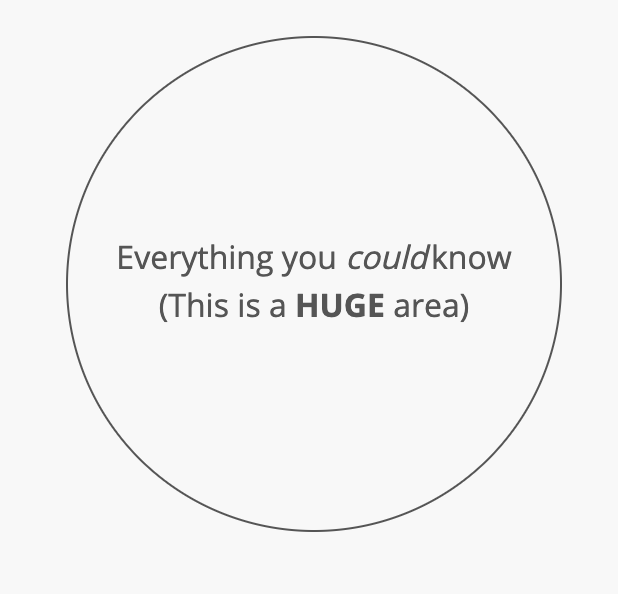
\includegraphics[width=0.5\textwidth]{pics/you-could-know}
  \caption{Everything you should know}
  \label{fig:you-could-know}
\end{figure}


In comparison to the vast world of things you could know, the stuff you actually know is just a tiny sliver. Shown in Figure \ref{fig:you-do-know}.

\begin{figure}[!ht]
  \centering
  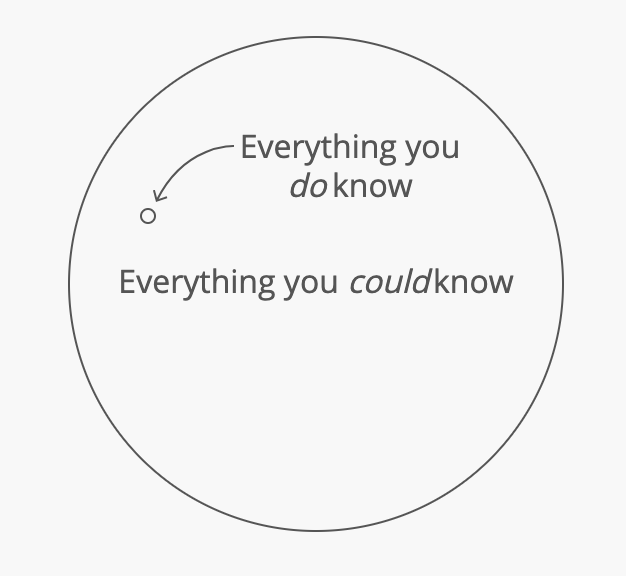
\includegraphics[width=0.5\textwidth]{pics/you-do-know}
  \caption{Everything you do know}
  \label{fig:you-do-know}
\end{figure}

 

That’s the first problem. \important{It feels like you don’t really know that much, because you only know a tiny sliver of all the stuff there is to know.}


\subsubsection{The expanding universe}

It gets worse: \important{counterintuitively, as you learn more, your sliver of knowledge feels like it's shrinking.}

That's because you brush up against more and more things you don’t know yet. Whole disciplines like machine learning, theory of computation, and embedded systems. Things you can't just pick up in an afternoon. Heavy bodies of knowledge that take months to understand.

So the universe of things you could know seems to keep expanding faster and faster—much faster than your tiny sliver of knowledge is growing. It feels like you'll never be able to keep up.


\subsubsection{What everyone else knows}

Here's another common cognitive bias: we assume that because something is easy for us, it must be easy for everyone else. So when we look at our own skills, we assume they're not unique. But when we look at other people's skills, we notice the skills they have that we don't have.

The result? We think everyone’s knowledge is a superset of our own (Figure \ref{fig:false-what-everyone-else-know}):

\begin{figure}[!ht]
  \centering
  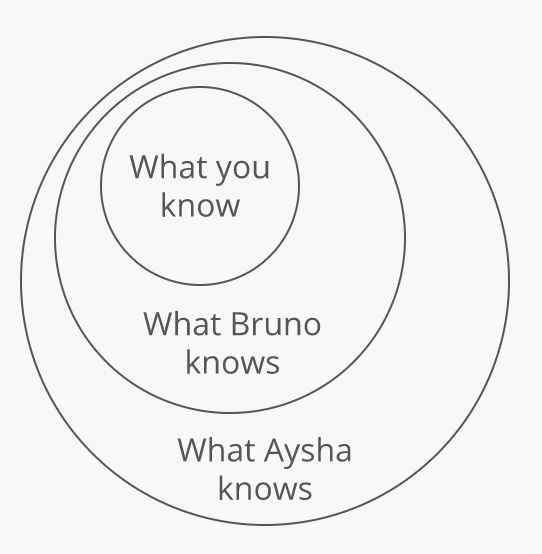
\includegraphics[width=0.5\textwidth]{pics/false-what-everyone-else-know}
  \label{fig:false-what-everyone-else-know}
\end{figure}


This makes us feel like everyone else is ahead of us. Like we're always a step behind.

But the truth is more like this (Figure \ref{fig:true-what-everyone-else-know}):

\begin{figure}[!ht]
  \centering
  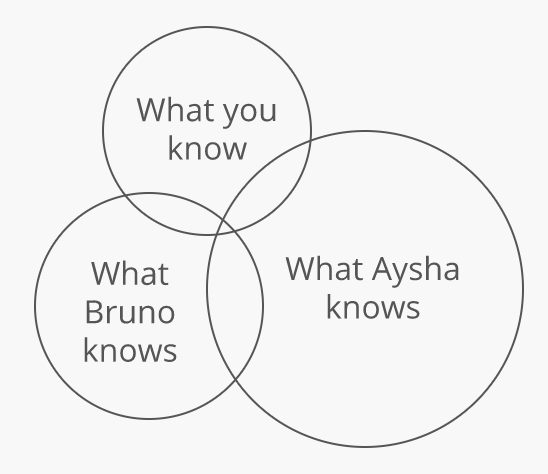
\includegraphics[width=0.5\textwidth]{pics/true-what-everyone-else-know}
  \label{fig:true-what-everyone-else-know}
\end{figure}


There's a whole area of stuff you know that neither Aysha nor Bruno knows. An area you're probably blind to, because you're so focused on the stuff you don't know.


\subsubsection{It's a problem of focus}

Focusing on what you don't know causes you to underestimate what you do know. And that's what causes impostor syndrome.

By looking at the vast (and expanding) universe of things you could know, you feel like you hardly know anything.

And by looking at what Aysha and Bruno know that you don't know, you feel like you're a step behind.

And interviews make you really focus on what you don't know. You focus on what could go wrong. The knowledge gaps your interviewers might find. The questions you might not know how to answer.

But remember:

Just because Aysha and Bruno know some things you don't know, doesn't mean you don't also know things Aysha and Bruno don't know.

And more importantly, everyone's body of knowledge is just a teeny-tiny sliver of everything they could learn. We all have gaps in our knowledge. We all have interview questions we won't be able to answer.

You're not a step behind. You just have a lot of stuff you don't know yet. Just like everyone else.



\subsection{Organizing Your Interview Timeline}

\subsubsection{Work backwards from a signing date}

\important{Pick a "signing date" and stick to it.}
This is the date that you plan to make a final decision and sign an offer. This includes some allowed time for negotiating once you have all your offers in hand (more on that later).

\subsubsection{How far out should my signing date be?}

It depends. At a high level, you should allow as much time as you can afford to. Most people underestimate how long their job search is going to take. And when you end up in a time crunch at the end, it means less time at the negotiation stage. So allowing an extra week for your job search could literally mean earning tens of thousands of dollars more in your final salary.

If you have a current job or are a full-time student, try to allow more time by starting the process earlier.

Of course, some of us will be in situations where we really need to start our new job as soon as possible. That's fine. Do what works for you.

Keep in mind that you’re shooting for having enough time to practice and get through the whole interview process with multiple companies if you can. Think through how much time you can devote to each of these steps:

\begin{itemize}
\item Studying (1–8 weeks)
\item Phone screens (1–3 weeks)
\item Onsites (1–3 weeks)
\item Negotiation (1–2 weeks)
\end{itemize}


One more consideration: if you have the means, consider leaving yourself some time for a vacation before starting your new job. Job hunting is stressful. And that window of time between signing a new offer and starting a new job can be a rare window of low stress and low responsibility in your life.



\subsubsection{Cast a wide net}

\important{Interview with multiple companies.} Exactly how many companies depends on your situation, but the point is to avoid putting all your eggs in one basket. You want multiple offers by the end, so you can negotiate the best offer possible.

A good rule of thumb: send out applications to more places than you’re currently planning. If you end up getting too many interviews…well that’s a good problem to have! You can always "pause" or simply cancel the interview process with some companies.

\important{Schedule your favorite companies last.} Get interview practice with the places you aren’t as excited about. You’ll be in your prime by the time you interview with your top choices, so long as you don’t burn out.

\important{Jot down your impressions after each interview.} You’ll be surprised how much different companies can start to melt together after a couple weeks of interviewing.


\subsubsection{Avoid burnout}

If you’re casting a wide net and allowing several weeks for your job search, you need to be careful about burnout. The interview process is a marathon, not a sprint.

\important{Space out your onsites.} Onsites are draining. Try to keep at least a two day buffer between them—one day to recover after your last onsite, and one day to get ready for the next.

\important{Don’t travel too much.} You can quickly burn yourself out bopping across the country. When you have to travel for an interview, try to wait a few days before you travel again.

Batch interviews that are in cities you have to fly to. Try to avoid flying to the same city multiple times—though sometimes traveling to the same place twice is better than trying to cram three or more onsites into a short span of time.


\subsection{Behavioral Questions}

\subsubsection{“Show, don’t tell”}

It’s good advice. When it comes to answering behavioral questions (like “Tell me about yourself”) in coding interviews, the difference between a good answer and a great answer comes down to showing rather than telling.


The problem is, people who give you the advice of “Show, don’t tell”… are themselves failing to follow it. They’re telling you to show, but they should be showing you how to show. That’s the hardest part!

So here are three specific tips for showing more and telling less.


\subsubsection{Sprinkle in specific details}

Imagine two responses to the stock interview question “Tell me about yourself.”

First:
\begin{tcolorbox}
I started programming about two years ago with some personal projects. I eventually got a job at a small tech company in my home town, and I’ve been working there about a year and a half. I like my job, but I’m looking for a new challenge, which I think your company could provide.  
\end{tcolorbox}


Then:
\begin{tcolorbox}
I got started programming because I wanted to build a social network for cats. That didn’t take off, but the prototype helped me get a job at a small tech company in my home town.

Last month, I read an awesome article on Hacker News about the social network your company is building. The scaling challenges you face seem like they’ll help me grow faster and stronger than my current role will.
\end{tcolorbox}



The second response says a lot more about the candidate.

Why? Because of the specific details. An interviewer won’t remember the tenth person to say “I’m looking for a new challenge.” They will remember the person who tried to build a social network for cats and read about their company on Hacker News.

So don’t skimp on the details. \important{Look out for opportunities to use specifics}, especially if they’re at all quirky, funny, surprising, or otherwise memorable.


\subsubsection{Tell a story from your life}

Take another common question: “Why do you want to work here?”

People tend to just cross-reference their values with those of the company or team they’re interviewing with:

\begin{tcolorbox}
I’m really interested in technical blogging and open source. So I like that your company has some open-source work and contributes back to the community.  
\end{tcolorbox}


That’s a fine response. But to really wow your interviewer, try adding a specific story around those values:

\begin{tcolorbox}
  A couple years ago, when I was still new to programming, I was working on this tricky bug. I found a post on a company blog where an engineer explained how her team solved the issue. She included a code snippet she’d open-sourced. I appreciated that she took the time to write about her team’s experience and share their solution. It helped me!

  That’s how I first started getting into open source. I really wanna work with more engineers like that—who write about their work and try to help others in the community. So I was excited to see all the stuff your team shares on your blog and on the company’s Github profile.
\end{tcolorbox}



The second response just sounds more genuine. It shows a personal connection to open source and technical blogging, instead of just telling it.

Anyone can look up a company’s core values and repeat them during an interview. It’s more meaningful to \important{tell a story from your life} that shows how those values benefited you or taught you something.



\subsubsection{Use someone else’s voice}

This one’s a neat trick. Consider one more standard behavioral question: “What’s your biggest strength?”

You might tell the interviewer:

\begin{tcolorbox}
I work well with others. Even under tough circumstances, I make sure my coworkers feel supported.  
\end{tcolorbox}


But a lightly detailed story is better suited to show this strength:

\begin{tcolorbox}
  I have a coworker, Ana, who’s been an engineer for almost a decade. We worked together on this really tough, messy project.

  Towards the end, she told me, “For such a hellish project, you really made things feel sane.” I think this is my biggest strength—I work well with others, even under tough circumstances.
\end{tcolorbox}

When you respond with a story, you can refer to what other people have said about your best qualities. In this case, a ten-year tech veteran said you made a project feel less awful. That kind of praise is a lot more credible when it comes from someone else.



\subsubsection{Practice, practice, practice}

Remember these specific tricks for showing rather than telling:

\begin{enumerate}
\item Use specific, memorable details. “Social network for cats” instead of “a personal project.”
\item Tell a story from your life. “I was trying to solve a tricky bug…” instead of “I value open source contributions.”
\item Use someone else’s voice. “’You really made things feel sane‘” instead of "I work well with others."
\end{enumerate}


Try these tactics out on the questions below. Keep in mind, sometimes it’s easiest to start with a “tell” response, then spruce it up to “show.”


\begin{itemize}
\item Tell me your biggest weakness as an engineer.
\item Describe a tricky bug you’ve encountered.
\item What’s the biggest project you’ve shipped?
\item What’s your favorite programming language? Why?
\item How do you overcome interpersonal conflicts with coworkers?
\end{itemize}



\end{document}

